\documentclass{article}

\title{Raspberry Pi report}
\date{2021-05-17}
\author{Steffen Geving}

\usepackage{graphicx}
\usepackage{apacite}
\usepackage[english]{babel}
\usepackage{url}


\begin{document}
\pagenumbering{gobble} % This disables page numbers on this page
\maketitle
    \begin{figure}[h!]
            \centering
            
\includegraphics[scale=0.5]{rpilogo.png}
            \caption{The official Raspberry Pi Foundation Logo}
            \label{fig:rpilogo}
    \end{figure}

    \begin{center}
        \vspace*{\fill}
        Raspberry Pi is a trademark of the Raspberry Pi Foundation.
        
    \end{center}
    \newpage

    \tableofcontents
    \newpage

    \section{The Raspberry Pi}
    The Raspberry Pi is a low-cost general purpose computer made to allow easy access into computing for students and children, as well as being a great tool for projects 
    that require a more complex computing platform than for example an MCU like the Atmel AVR yet still being easy to use unlike an FPGA. ~\cite{RaspberryPi}

    \section{The need for a low-cost general purpose computer}
    The Raspberry Pi was started because the creator felt there was a need for a cheap computer that people could learn with, similar to the BBC micro in the eighties. 
    The Raspberry Pi is the brainchild of Eben Upton. Inspired by the computer of his childhood, the BBC Micro, he felt there was a need for a similar solution for students 
    and children of today.
    \begin{quotation}
     "Dr Upton and colleagues at the Cambridge Computer Laboratory had been concerned at the declining figures for young people interested in computer science."
     % WHY DO YOU BREAK EVERYTHING \cite{EbenUpton}
    \end{quotation} 
    So he set out to make a general purpose computer that would be easy to use and also be low cost, as to be available to developing countries too. To aid in his design for his computer he consulted teachers, computer hobbyists and academics and put together a group aimed at devising his dream to inspire children to get into computing.

    \section{The history of the Raspberry Pi}
    \begin{figure}[ht]
        \centering
        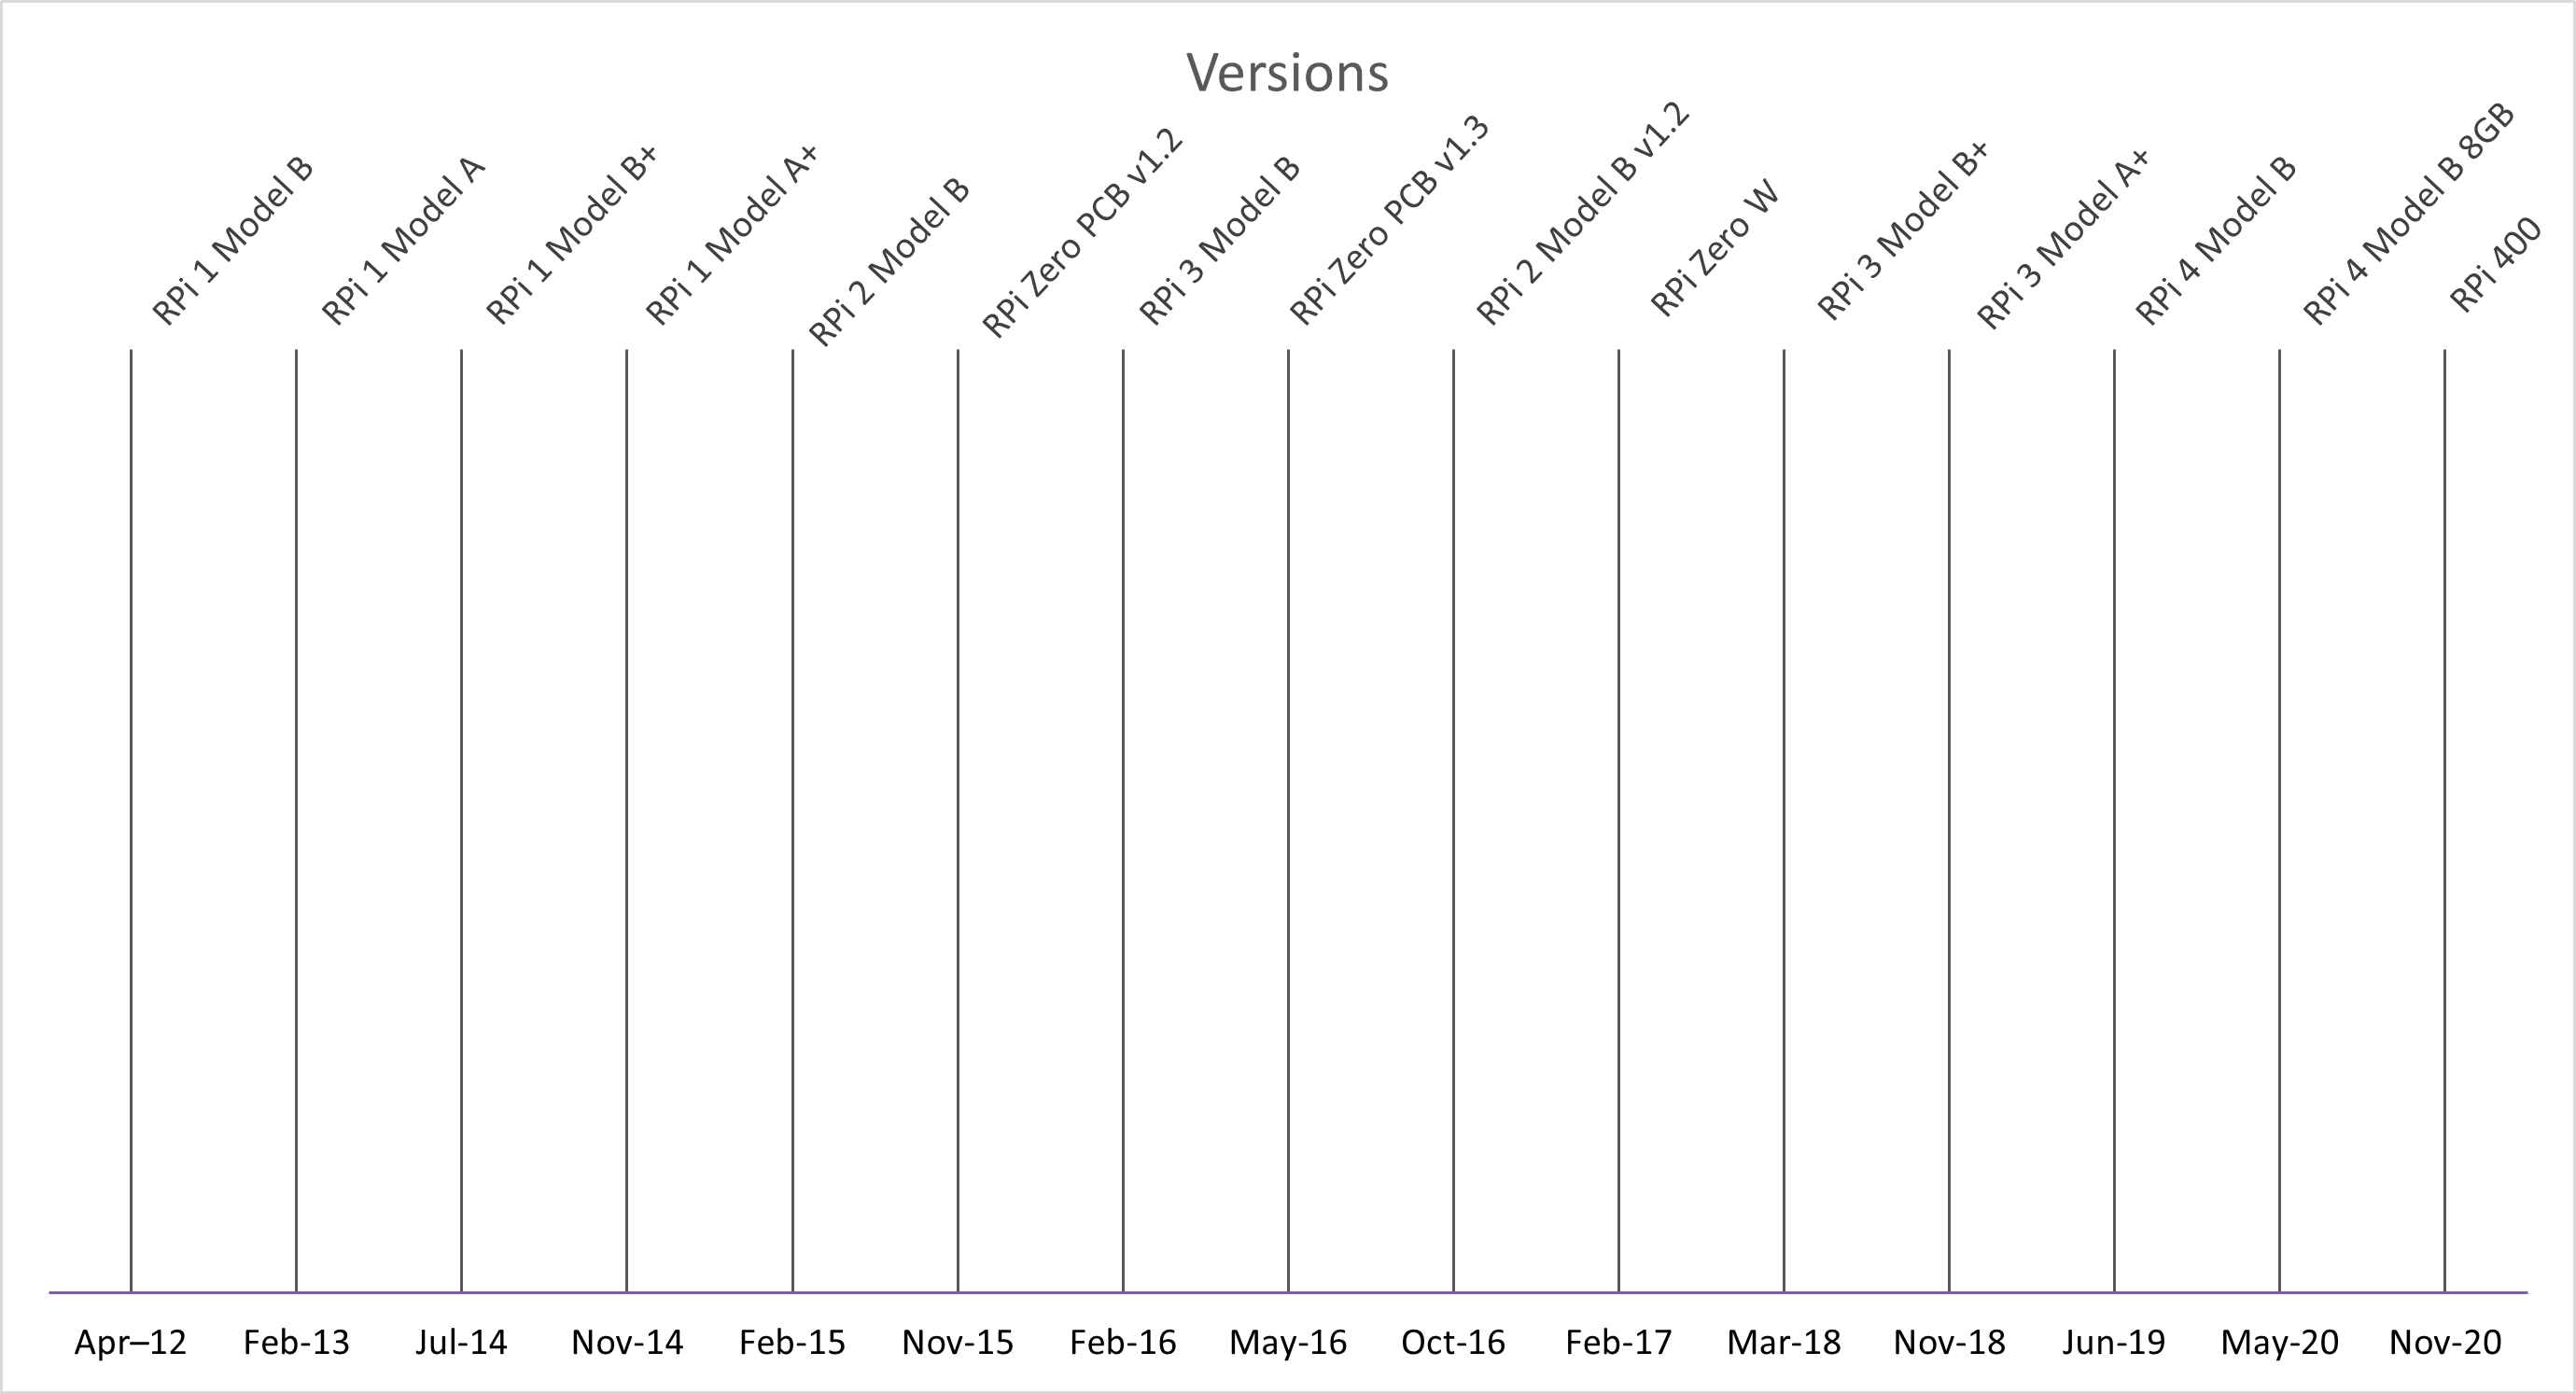
\includegraphics[scale=0.4]{versions.png}
        \caption{Timeline of the Raspberry Pi versions}
        \label{fig:rpiver}
    \end{figure}

    \newpage


    \section{The operating systems of the Raspberry Pi}
    You can put any operating system that compiles for ARMv6-32 RPi1 bit or ARMv7-32 bit RPi 2 v1.1 ARMv8-64 bit RPi 2 v1.2 and latter models. The offical operating system for the 
    Raspberry Pi is Raspberry Pi OS (formerly Rasbian). According to the website distrowatch.com the top 3 distributions for the Raspberry Pi by popularity are MX Linux, Manjaro Linux 
    and openSUSE.

    \section{Raspberry Pi MSRPs}
    These are the recommended prices for the various Raspberry Pi models as set by the Raspberry Pi Foundation~\cite{RaspberryPiPrice}

    \begin{center}
        \begin{tabular}{ |c|c| } 
            \hline
            Model & Price \\
            \hline\hline
            Raspberry Pi Model A & \$25 \\
            \hline
            Raspberry Pi Model A+ & \$20 \\
            \hline
            Raspberry Pi 3 Model A+	& \$25 \\
            \hline
            Raspberry Pi Model B & \$35 \\
            \hline
            Raspberry Pi Model B+ & \$25 \\
            \hline
            Raspberry Pi 2 Model B & \$35 \\
            \hline
            Raspberry Pi Model B v1.2 & \$35 \\
            \hline
            Raspberry Pi 3 Model B & \$35 \\
            \hline
            Raspberry Pi 3 Model B+ & \$35 \\
            \hline
            Raspberry Pi 4 Model B & \$35\textsuperscript{\textdagger}\\
            \hline
            Raspberry Pi Zero PCB v1.3 & \$5 \\
            \hline
            Raspberry Pi Zero W & \$10 \\
            \hline
            Raspberry Pi 400 & \$70 \\
            \hline
        \end{tabular}
    \end{center}
    \textsuperscript{\textdagger}Prices vary for different RAM configurations
     \$35 (2GB RAM), \$55 (4GB RAM), \$75 (8GB RAM) 

    \section{Differences between the Raspberry Pi and other integrated circuitry}
    The Raspberry Pi is a general purpose computer, meaning that it is designed to be plugged into various human input and output devices and be directly influenced by a human being. 
    And that it runs an operating system that you can install software on. Microcontrollers (MCUs) on the other hand are more bare-bone and need a pre-compiled software image flashed
    directly on to the chip. Or it needs a boot-loader so that it can boot up and read its program from a storage device. Examples are the Micro:Bit and Arduino microcontrollers. 
    A microprocessor is similar to a microcontroller in the fact that it needs a program to be pre-compiled anytime you want it to run differently, but microprocessors also lack 
    many features that MCUs have. Like integrated RAM, various I/O devices. Microprocessors are designed to be used in conjunction with other discrete integrated circuits.

    \section{Raspberry Pi use cases}
    Raspberry Pis can be used for anything from a Personal Computer to a lightswitch. Many people use the Raspberry Pi as an arcade game emulator and build them into tabletop 
    arcade machines or arcade controllers. Another popular use for the Raspberry Pi is in robotics as its generious GPIO headers allow for many sensors and motors to be controlled. 
    Personally I have used my Raspberry Pi as a security camera with Raspbian and the software Motion~\cite{Motion}
    Some uses for the Raspberry Pi I found in my research was this paper ~\cite{KhatriPunit2019RPss} that proposes a hardware platform to be made that uses the Raspberry Pi, 
    to monitor and report water quality in real time. In Greenhills School, Michigan, USA, they have Raspberry Pi kits available for students to check out of the library to use for 
    projects in the classroom or at home~\cite{Toth-CherninJan2015RP}

    \section{Best use case for a Raspberry Pi}
    In my opinion the best use of a Raspberry Pi is in teaching young people computing. As PCs today are a behemoth of abstraction over unfathomably complex electric circuitry. 
    As Greenhills School discovered when they added Raspberry Pi kits to their library as items to check out. And they saw students were able to intuitively understand what 
    they were doing to the point where they were teaching and collaborating with other students. ~\cite{Toth-CherninJan2015RP}


    
    \bibliographystyle{apacite}
    \bibliography{bibtex/report}
\end{document}